\documentclass[twoside]{book}

% Packages required by doxygen
\usepackage{fixltx2e}
\usepackage{calc}
\usepackage{doxygen}
\usepackage[export]{adjustbox} % also loads graphicx
\usepackage{graphicx}
\usepackage[utf8]{inputenc}
\usepackage{makeidx}
\usepackage{multicol}
\usepackage{multirow}
\PassOptionsToPackage{warn}{textcomp}
\usepackage{textcomp}
\usepackage[nointegrals]{wasysym}
\usepackage[table]{xcolor}

% Font selection
\usepackage[T1]{fontenc}
\usepackage[scaled=.90]{helvet}
\usepackage{courier}
\usepackage{amssymb}
\usepackage{sectsty}
\renewcommand{\familydefault}{\sfdefault}
\allsectionsfont{%
  \fontseries{bc}\selectfont%
  \color{darkgray}%
}
\renewcommand{\DoxyLabelFont}{%
  \fontseries{bc}\selectfont%
  \color{darkgray}%
}
\newcommand{\+}{\discretionary{\mbox{\scriptsize$\hookleftarrow$}}{}{}}

% Page & text layout
\usepackage{geometry}
\geometry{%
  a4paper,%
  top=2.5cm,%
  bottom=2.5cm,%
  left=2.5cm,%
  right=2.5cm%
}
\tolerance=750
\hfuzz=15pt
\hbadness=750
\setlength{\emergencystretch}{15pt}
\setlength{\parindent}{0cm}
\setlength{\parskip}{3ex plus 2ex minus 2ex}
\makeatletter
\renewcommand{\paragraph}{%
  \@startsection{paragraph}{4}{0ex}{-1.0ex}{1.0ex}{%
    \normalfont\normalsize\bfseries\SS@parafont%
  }%
}
\renewcommand{\subparagraph}{%
  \@startsection{subparagraph}{5}{0ex}{-1.0ex}{1.0ex}{%
    \normalfont\normalsize\bfseries\SS@subparafont%
  }%
}
\makeatother

% Headers & footers
\usepackage{fancyhdr}
\pagestyle{fancyplain}
\fancyhead[LE]{\fancyplain{}{\bfseries\thepage}}
\fancyhead[CE]{\fancyplain{}{}}
\fancyhead[RE]{\fancyplain{}{\bfseries\leftmark}}
\fancyhead[LO]{\fancyplain{}{\bfseries\rightmark}}
\fancyhead[CO]{\fancyplain{}{}}
\fancyhead[RO]{\fancyplain{}{\bfseries\thepage}}
\fancyfoot[LE]{\fancyplain{}{}}
\fancyfoot[CE]{\fancyplain{}{}}
\fancyfoot[RE]{\fancyplain{}{\bfseries\scriptsize Generated by Doxygen }}
\fancyfoot[LO]{\fancyplain{}{\bfseries\scriptsize Generated by Doxygen }}
\fancyfoot[CO]{\fancyplain{}{}}
\fancyfoot[RO]{\fancyplain{}{}}
\renewcommand{\footrulewidth}{0.4pt}
\renewcommand{\chaptermark}[1]{%
  \markboth{#1}{}%
}
\renewcommand{\sectionmark}[1]{%
  \markright{\thesection\ #1}%
}

% Indices & bibliography
\usepackage{natbib}
\usepackage[titles]{tocloft}
\setcounter{tocdepth}{3}
\setcounter{secnumdepth}{5}
\makeindex

% Hyperlinks (required, but should be loaded last)
\usepackage{ifpdf}
\ifpdf
  \usepackage[pdftex,pagebackref=true]{hyperref}
\else
  \usepackage[ps2pdf,pagebackref=true]{hyperref}
\fi
\hypersetup{%
  colorlinks=true,%
  linkcolor=blue,%
  citecolor=blue,%
  unicode%
}

% Custom commands
\newcommand{\clearemptydoublepage}{%
  \newpage{\pagestyle{empty}\cleardoublepage}%
}

\usepackage{caption}
\captionsetup{labelsep=space,justification=centering,font={bf},singlelinecheck=off,skip=4pt,position=top}

%===== C O N T E N T S =====

\begin{document}

% Titlepage & ToC
\hypersetup{pageanchor=false,
             bookmarksnumbered=true,
             pdfencoding=unicode
            }
\pagenumbering{alph}
\begin{titlepage}
\vspace*{7cm}
\begin{center}%
{\Large My Project \\[1ex]\large 1 }\\
\vspace*{1cm}
{\large Generated by Doxygen 1.8.13}\\
\end{center}
\end{titlepage}
\clearemptydoublepage
\pagenumbering{roman}
\tableofcontents
\clearemptydoublepage
\pagenumbering{arabic}
\hypersetup{pageanchor=true}

%--- Begin generated contents ---
\chapter{Class Index}
\section{Class List}
Here are the classes, structs, unions and interfaces with brief descriptions\+:\begin{DoxyCompactList}
\item\contentsline{section}{\hyperlink{class_a_v_l_tree}{A\+V\+L\+Tree} \\*Class for A\+VL Tree }{\pageref{class_a_v_l_tree}}{}
\item\contentsline{section}{\hyperlink{structnode}{node} }{\pageref{structnode}}{}
\item\contentsline{section}{\hyperlink{class_node}{Node} }{\pageref{class_node}}{}
\item\contentsline{section}{\hyperlink{struct_r_b_t_node}{R\+B\+T\+Node} \\*\hyperlink{struct_r_b_t_node}{R\+B\+T\+Node} for red black tree }{\pageref{struct_r_b_t_node}}{}
\item\contentsline{section}{\hyperlink{class_r_b_tree}{R\+B\+Tree} \\*Class to represent Red-\/\+Black Tree }{\pageref{class_r_b_tree}}{}
\end{DoxyCompactList}

\chapter{File Index}
\section{File List}
Here is a list of all files with brief descriptions\+:\begin{DoxyCompactList}
\item\contentsline{section}{/home/kavya/\+Desktop/csn261\+\_\+lab\+\_\+assignment1/q1/code/\hyperlink{q1_8c}{q1.\+c} }{\pageref{q1_8c}}{}
\end{DoxyCompactList}

\chapter{Class Documentation}
\hypertarget{class_fibonacci_heap}{}\section{Fibonacci\+Heap$<$ V $>$ Class Template Reference}
\label{class_fibonacci_heap}\index{Fibonacci\+Heap$<$ V $>$@{Fibonacci\+Heap$<$ V $>$}}


{\ttfamily \#include $<$fibonacci\+\_\+heap.\+h$>$}

\subsection*{Public Member Functions}
\begin{DoxyCompactItemize}
\item 
\hyperlink{class_fibonacci_heap_ab59b6ac11eaf6f956b4e3db7d8c3c472}{Fibonacci\+Heap} ()
\item 
\hyperlink{class_fibonacci_heap_a106b353a0c16a47d28916cac8b2370a0}{$\sim$\+Fibonacci\+Heap} ()
\item 
void \hyperlink{class_fibonacci_heap_a2726ce00ae9e20ef8bd88a1bf2f41313}{delete\+All} (\hyperlink{structnode}{node}$<$ V $>$ $\ast$n)
\item 
\hyperlink{structnode}{node}$<$ V $>$ $\ast$ \hyperlink{class_fibonacci_heap_a2de69d27315f0f4cd6c2375a485c6ef5}{create\+\_\+node} (V value)
\item 
\hyperlink{structnode}{node}$<$ V $>$ $\ast$ \hyperlink{class_fibonacci_heap_a131874fb70c0ed4b2a09b94afa71ed6a}{merge\+\_\+heaps} (\hyperlink{structnode}{node}$<$ V $>$ $\ast$a, \hyperlink{structnode}{node}$<$ V $>$ $\ast$b)
\item 
\hyperlink{structnode}{node}$<$ V $>$ $\ast$ \hyperlink{class_fibonacci_heap_a0f46f3062277aecb53bfbaa92d35a765}{insert} (V value)
\item 
V \hyperlink{class_fibonacci_heap_a63cc52318444c719a45f75a3b0698d31}{get\+\_\+min} ()
\item 
void \hyperlink{class_fibonacci_heap_aa9ad54a64b54264ec3dd435a4190af16}{add\+Child} (\hyperlink{structnode}{node}$<$ V $>$ $\ast$parent, \hyperlink{structnode}{node}$<$ V $>$ $\ast$child)
\item 
\hyperlink{structnode}{node}$<$ V $>$ $\ast$ \hyperlink{class_fibonacci_heap_a0ce9ea86a726ae81bcd8935bff6dc954}{extract\+\_\+min\+\_\+helper} (\hyperlink{structnode}{node}$<$ V $>$ $\ast$n)
\item 
V \hyperlink{class_fibonacci_heap_ad483e2607e101d410781fb52bb3099ac}{extract\+\_\+min} ()
\item 
\hyperlink{structnode}{node}$<$ V $>$ $\ast$ \hyperlink{class_fibonacci_heap_a215c1e3fbf82b73f7548ef9b2e4420e3}{find\+\_\+helper} (\hyperlink{structnode}{node}$<$ V $>$ $\ast$\hyperlink{class_fibonacci_heap_a13c58cd79d84a4398fb9fb1c956ccfc5}{heap}, V value)
\item 
\hyperlink{structnode}{node}$<$ V $>$ $\ast$ \hyperlink{class_fibonacci_heap_ae6083007b440bd41d8adbd44c9bb7636}{find} (V value)
\item 
\hyperlink{structnode}{node}$<$ V $>$ $\ast$ \hyperlink{class_fibonacci_heap_a6777625b9569bd48fcefa848d7a8812a}{cut} (\hyperlink{structnode}{node}$<$ V $>$ $\ast$\hyperlink{class_fibonacci_heap_a13c58cd79d84a4398fb9fb1c956ccfc5}{heap}, \hyperlink{structnode}{node}$<$ V $>$ $\ast$n)
\item 
\hyperlink{structnode}{node}$<$ V $>$ $\ast$ \hyperlink{class_fibonacci_heap_ab97deb5ff0e3944eba71a1ba5d99d2b6}{decrease\+\_\+key\+\_\+helper} (\hyperlink{structnode}{node}$<$ V $>$ $\ast$\hyperlink{class_fibonacci_heap_a13c58cd79d84a4398fb9fb1c956ccfc5}{heap}, \hyperlink{structnode}{node}$<$ V $>$ $\ast$n, V value)
\item 
void \hyperlink{class_fibonacci_heap_a36e1518c83aa296c0c8b9a6e4cfb42d6}{decrease\+\_\+key} (V i, V value)
\end{DoxyCompactItemize}
\subsection*{Public Attributes}
\begin{DoxyCompactItemize}
\item 
\hyperlink{structnode}{node}$<$ V $>$ $\ast$ \hyperlink{class_fibonacci_heap_a13c58cd79d84a4398fb9fb1c956ccfc5}{heap}
\end{DoxyCompactItemize}


\subsection{Detailed Description}
\subsubsection*{template$<$class V$>$\newline
class Fibonacci\+Heap$<$ V $>$}



Definition at line 16 of file fibonacci\+\_\+heap.\+h.



\subsection{Constructor \& Destructor Documentation}
\mbox{\Hypertarget{class_fibonacci_heap_ab59b6ac11eaf6f956b4e3db7d8c3c472}\label{class_fibonacci_heap_ab59b6ac11eaf6f956b4e3db7d8c3c472}} 
\index{Fibonacci\+Heap@{Fibonacci\+Heap}!Fibonacci\+Heap@{Fibonacci\+Heap}}
\index{Fibonacci\+Heap@{Fibonacci\+Heap}!Fibonacci\+Heap@{Fibonacci\+Heap}}
\subsubsection{\texorpdfstring{Fibonacci\+Heap()}{FibonacciHeap()}}
{\footnotesize\ttfamily template$<$class V$>$ \\
\hyperlink{class_fibonacci_heap}{Fibonacci\+Heap}$<$ V $>$\+::\hyperlink{class_fibonacci_heap}{Fibonacci\+Heap} (\begin{DoxyParamCaption}{ }\end{DoxyParamCaption})\hspace{0.3cm}{\ttfamily [inline]}}



Definition at line 21 of file fibonacci\+\_\+heap.\+h.

\mbox{\Hypertarget{class_fibonacci_heap_a106b353a0c16a47d28916cac8b2370a0}\label{class_fibonacci_heap_a106b353a0c16a47d28916cac8b2370a0}} 
\index{Fibonacci\+Heap@{Fibonacci\+Heap}!````~Fibonacci\+Heap@{$\sim$\+Fibonacci\+Heap}}
\index{````~Fibonacci\+Heap@{$\sim$\+Fibonacci\+Heap}!Fibonacci\+Heap@{Fibonacci\+Heap}}
\subsubsection{\texorpdfstring{$\sim$\+Fibonacci\+Heap()}{~FibonacciHeap()}}
{\footnotesize\ttfamily template$<$class V$>$ \\
\hyperlink{class_fibonacci_heap}{Fibonacci\+Heap}$<$ V $>$\+::$\sim$\hyperlink{class_fibonacci_heap}{Fibonacci\+Heap} (\begin{DoxyParamCaption}{ }\end{DoxyParamCaption})\hspace{0.3cm}{\ttfamily [inline]}}



Definition at line 26 of file fibonacci\+\_\+heap.\+h.



\subsection{Member Function Documentation}
\mbox{\Hypertarget{class_fibonacci_heap_aa9ad54a64b54264ec3dd435a4190af16}\label{class_fibonacci_heap_aa9ad54a64b54264ec3dd435a4190af16}} 
\index{Fibonacci\+Heap@{Fibonacci\+Heap}!add\+Child@{add\+Child}}
\index{add\+Child@{add\+Child}!Fibonacci\+Heap@{Fibonacci\+Heap}}
\subsubsection{\texorpdfstring{add\+Child()}{addChild()}}
{\footnotesize\ttfamily template$<$class V$>$ \\
void \hyperlink{class_fibonacci_heap}{Fibonacci\+Heap}$<$ V $>$\+::add\+Child (\begin{DoxyParamCaption}\item[{\hyperlink{structnode}{node}$<$ V $>$ $\ast$}]{parent,  }\item[{\hyperlink{structnode}{node}$<$ V $>$ $\ast$}]{child }\end{DoxyParamCaption})\hspace{0.3cm}{\ttfamily [inline]}}



Definition at line 97 of file fibonacci\+\_\+heap.\+h.

\mbox{\Hypertarget{class_fibonacci_heap_a2de69d27315f0f4cd6c2375a485c6ef5}\label{class_fibonacci_heap_a2de69d27315f0f4cd6c2375a485c6ef5}} 
\index{Fibonacci\+Heap@{Fibonacci\+Heap}!create\+\_\+node@{create\+\_\+node}}
\index{create\+\_\+node@{create\+\_\+node}!Fibonacci\+Heap@{Fibonacci\+Heap}}
\subsubsection{\texorpdfstring{create\+\_\+node()}{create\_node()}}
{\footnotesize\ttfamily template$<$class V$>$ \\
\hyperlink{structnode}{node}$<$V$>$$\ast$ \hyperlink{class_fibonacci_heap}{Fibonacci\+Heap}$<$ V $>$\+::create\+\_\+node (\begin{DoxyParamCaption}\item[{V}]{value }\end{DoxyParamCaption})\hspace{0.3cm}{\ttfamily [inline]}}



Definition at line 49 of file fibonacci\+\_\+heap.\+h.

\mbox{\Hypertarget{class_fibonacci_heap_a6777625b9569bd48fcefa848d7a8812a}\label{class_fibonacci_heap_a6777625b9569bd48fcefa848d7a8812a}} 
\index{Fibonacci\+Heap@{Fibonacci\+Heap}!cut@{cut}}
\index{cut@{cut}!Fibonacci\+Heap@{Fibonacci\+Heap}}
\subsubsection{\texorpdfstring{cut()}{cut()}}
{\footnotesize\ttfamily template$<$class V$>$ \\
\hyperlink{structnode}{node}$<$V$>$$\ast$ \hyperlink{class_fibonacci_heap}{Fibonacci\+Heap}$<$ V $>$\+::cut (\begin{DoxyParamCaption}\item[{\hyperlink{structnode}{node}$<$ V $>$ $\ast$}]{heap,  }\item[{\hyperlink{structnode}{node}$<$ V $>$ $\ast$}]{n }\end{DoxyParamCaption})\hspace{0.3cm}{\ttfamily [inline]}}



Definition at line 223 of file fibonacci\+\_\+heap.\+h.

\mbox{\Hypertarget{class_fibonacci_heap_a36e1518c83aa296c0c8b9a6e4cfb42d6}\label{class_fibonacci_heap_a36e1518c83aa296c0c8b9a6e4cfb42d6}} 
\index{Fibonacci\+Heap@{Fibonacci\+Heap}!decrease\+\_\+key@{decrease\+\_\+key}}
\index{decrease\+\_\+key@{decrease\+\_\+key}!Fibonacci\+Heap@{Fibonacci\+Heap}}
\subsubsection{\texorpdfstring{decrease\+\_\+key()}{decrease\_key()}}
{\footnotesize\ttfamily template$<$class V$>$ \\
void \hyperlink{class_fibonacci_heap}{Fibonacci\+Heap}$<$ V $>$\+::decrease\+\_\+key (\begin{DoxyParamCaption}\item[{V}]{i,  }\item[{V}]{value }\end{DoxyParamCaption})\hspace{0.3cm}{\ttfamily [inline]}}



Definition at line 273 of file fibonacci\+\_\+heap.\+h.

\mbox{\Hypertarget{class_fibonacci_heap_ab97deb5ff0e3944eba71a1ba5d99d2b6}\label{class_fibonacci_heap_ab97deb5ff0e3944eba71a1ba5d99d2b6}} 
\index{Fibonacci\+Heap@{Fibonacci\+Heap}!decrease\+\_\+key\+\_\+helper@{decrease\+\_\+key\+\_\+helper}}
\index{decrease\+\_\+key\+\_\+helper@{decrease\+\_\+key\+\_\+helper}!Fibonacci\+Heap@{Fibonacci\+Heap}}
\subsubsection{\texorpdfstring{decrease\+\_\+key\+\_\+helper()}{decrease\_key\_helper()}}
{\footnotesize\ttfamily template$<$class V$>$ \\
\hyperlink{structnode}{node}$<$V$>$$\ast$ \hyperlink{class_fibonacci_heap}{Fibonacci\+Heap}$<$ V $>$\+::decrease\+\_\+key\+\_\+helper (\begin{DoxyParamCaption}\item[{\hyperlink{structnode}{node}$<$ V $>$ $\ast$}]{heap,  }\item[{\hyperlink{structnode}{node}$<$ V $>$ $\ast$}]{n,  }\item[{V}]{value }\end{DoxyParamCaption})\hspace{0.3cm}{\ttfamily [inline]}}



Definition at line 240 of file fibonacci\+\_\+heap.\+h.

\mbox{\Hypertarget{class_fibonacci_heap_a2726ce00ae9e20ef8bd88a1bf2f41313}\label{class_fibonacci_heap_a2726ce00ae9e20ef8bd88a1bf2f41313}} 
\index{Fibonacci\+Heap@{Fibonacci\+Heap}!delete\+All@{delete\+All}}
\index{delete\+All@{delete\+All}!Fibonacci\+Heap@{Fibonacci\+Heap}}
\subsubsection{\texorpdfstring{delete\+All()}{deleteAll()}}
{\footnotesize\ttfamily template$<$class V$>$ \\
void \hyperlink{class_fibonacci_heap}{Fibonacci\+Heap}$<$ V $>$\+::delete\+All (\begin{DoxyParamCaption}\item[{\hyperlink{structnode}{node}$<$ V $>$ $\ast$}]{n }\end{DoxyParamCaption})\hspace{0.3cm}{\ttfamily [inline]}}



Definition at line 34 of file fibonacci\+\_\+heap.\+h.

\mbox{\Hypertarget{class_fibonacci_heap_ad483e2607e101d410781fb52bb3099ac}\label{class_fibonacci_heap_ad483e2607e101d410781fb52bb3099ac}} 
\index{Fibonacci\+Heap@{Fibonacci\+Heap}!extract\+\_\+min@{extract\+\_\+min}}
\index{extract\+\_\+min@{extract\+\_\+min}!Fibonacci\+Heap@{Fibonacci\+Heap}}
\subsubsection{\texorpdfstring{extract\+\_\+min()}{extract\_min()}}
{\footnotesize\ttfamily template$<$class V$>$ \\
V \hyperlink{class_fibonacci_heap}{Fibonacci\+Heap}$<$ V $>$\+::extract\+\_\+min (\begin{DoxyParamCaption}{ }\end{DoxyParamCaption})\hspace{0.3cm}{\ttfamily [inline]}}



Definition at line 190 of file fibonacci\+\_\+heap.\+h.

\mbox{\Hypertarget{class_fibonacci_heap_a0ce9ea86a726ae81bcd8935bff6dc954}\label{class_fibonacci_heap_a0ce9ea86a726ae81bcd8935bff6dc954}} 
\index{Fibonacci\+Heap@{Fibonacci\+Heap}!extract\+\_\+min\+\_\+helper@{extract\+\_\+min\+\_\+helper}}
\index{extract\+\_\+min\+\_\+helper@{extract\+\_\+min\+\_\+helper}!Fibonacci\+Heap@{Fibonacci\+Heap}}
\subsubsection{\texorpdfstring{extract\+\_\+min\+\_\+helper()}{extract\_min\_helper()}}
{\footnotesize\ttfamily template$<$class V$>$ \\
\hyperlink{structnode}{node}$<$V$>$$\ast$ \hyperlink{class_fibonacci_heap}{Fibonacci\+Heap}$<$ V $>$\+::extract\+\_\+min\+\_\+helper (\begin{DoxyParamCaption}\item[{\hyperlink{structnode}{node}$<$ V $>$ $\ast$}]{n }\end{DoxyParamCaption})\hspace{0.3cm}{\ttfamily [inline]}}



Definition at line 105 of file fibonacci\+\_\+heap.\+h.

\mbox{\Hypertarget{class_fibonacci_heap_ae6083007b440bd41d8adbd44c9bb7636}\label{class_fibonacci_heap_ae6083007b440bd41d8adbd44c9bb7636}} 
\index{Fibonacci\+Heap@{Fibonacci\+Heap}!find@{find}}
\index{find@{find}!Fibonacci\+Heap@{Fibonacci\+Heap}}
\subsubsection{\texorpdfstring{find()}{find()}}
{\footnotesize\ttfamily template$<$class V$>$ \\
\hyperlink{structnode}{node}$<$V$>$$\ast$ \hyperlink{class_fibonacci_heap}{Fibonacci\+Heap}$<$ V $>$\+::find (\begin{DoxyParamCaption}\item[{V}]{value }\end{DoxyParamCaption})\hspace{0.3cm}{\ttfamily [inline]}}



Definition at line 218 of file fibonacci\+\_\+heap.\+h.

\mbox{\Hypertarget{class_fibonacci_heap_a215c1e3fbf82b73f7548ef9b2e4420e3}\label{class_fibonacci_heap_a215c1e3fbf82b73f7548ef9b2e4420e3}} 
\index{Fibonacci\+Heap@{Fibonacci\+Heap}!find\+\_\+helper@{find\+\_\+helper}}
\index{find\+\_\+helper@{find\+\_\+helper}!Fibonacci\+Heap@{Fibonacci\+Heap}}
\subsubsection{\texorpdfstring{find\+\_\+helper()}{find\_helper()}}
{\footnotesize\ttfamily template$<$class V$>$ \\
\hyperlink{structnode}{node}$<$V$>$$\ast$ \hyperlink{class_fibonacci_heap}{Fibonacci\+Heap}$<$ V $>$\+::find\+\_\+helper (\begin{DoxyParamCaption}\item[{\hyperlink{structnode}{node}$<$ V $>$ $\ast$}]{heap,  }\item[{V}]{value }\end{DoxyParamCaption})\hspace{0.3cm}{\ttfamily [inline]}}



Definition at line 201 of file fibonacci\+\_\+heap.\+h.

\mbox{\Hypertarget{class_fibonacci_heap_a63cc52318444c719a45f75a3b0698d31}\label{class_fibonacci_heap_a63cc52318444c719a45f75a3b0698d31}} 
\index{Fibonacci\+Heap@{Fibonacci\+Heap}!get\+\_\+min@{get\+\_\+min}}
\index{get\+\_\+min@{get\+\_\+min}!Fibonacci\+Heap@{Fibonacci\+Heap}}
\subsubsection{\texorpdfstring{get\+\_\+min()}{get\_min()}}
{\footnotesize\ttfamily template$<$class V$>$ \\
V \hyperlink{class_fibonacci_heap}{Fibonacci\+Heap}$<$ V $>$\+::get\+\_\+min (\begin{DoxyParamCaption}{ }\end{DoxyParamCaption})\hspace{0.3cm}{\ttfamily [inline]}}



Definition at line 89 of file fibonacci\+\_\+heap.\+h.

\mbox{\Hypertarget{class_fibonacci_heap_a0f46f3062277aecb53bfbaa92d35a765}\label{class_fibonacci_heap_a0f46f3062277aecb53bfbaa92d35a765}} 
\index{Fibonacci\+Heap@{Fibonacci\+Heap}!insert@{insert}}
\index{insert@{insert}!Fibonacci\+Heap@{Fibonacci\+Heap}}
\subsubsection{\texorpdfstring{insert()}{insert()}}
{\footnotesize\ttfamily template$<$class V$>$ \\
\hyperlink{structnode}{node}$<$V$>$$\ast$ \hyperlink{class_fibonacci_heap}{Fibonacci\+Heap}$<$ V $>$\+::insert (\begin{DoxyParamCaption}\item[{V}]{value }\end{DoxyParamCaption})\hspace{0.3cm}{\ttfamily [inline]}}



Definition at line 82 of file fibonacci\+\_\+heap.\+h.

\mbox{\Hypertarget{class_fibonacci_heap_a131874fb70c0ed4b2a09b94afa71ed6a}\label{class_fibonacci_heap_a131874fb70c0ed4b2a09b94afa71ed6a}} 
\index{Fibonacci\+Heap@{Fibonacci\+Heap}!merge\+\_\+heaps@{merge\+\_\+heaps}}
\index{merge\+\_\+heaps@{merge\+\_\+heaps}!Fibonacci\+Heap@{Fibonacci\+Heap}}
\subsubsection{\texorpdfstring{merge\+\_\+heaps()}{merge\_heaps()}}
{\footnotesize\ttfamily template$<$class V$>$ \\
\hyperlink{structnode}{node}$<$V$>$$\ast$ \hyperlink{class_fibonacci_heap}{Fibonacci\+Heap}$<$ V $>$\+::merge\+\_\+heaps (\begin{DoxyParamCaption}\item[{\hyperlink{structnode}{node}$<$ V $>$ $\ast$}]{a,  }\item[{\hyperlink{structnode}{node}$<$ V $>$ $\ast$}]{b }\end{DoxyParamCaption})\hspace{0.3cm}{\ttfamily [inline]}}



Definition at line 61 of file fibonacci\+\_\+heap.\+h.



\subsection{Member Data Documentation}
\mbox{\Hypertarget{class_fibonacci_heap_a13c58cd79d84a4398fb9fb1c956ccfc5}\label{class_fibonacci_heap_a13c58cd79d84a4398fb9fb1c956ccfc5}} 
\index{Fibonacci\+Heap@{Fibonacci\+Heap}!heap@{heap}}
\index{heap@{heap}!Fibonacci\+Heap@{Fibonacci\+Heap}}
\subsubsection{\texorpdfstring{heap}{heap}}
{\footnotesize\ttfamily template$<$class V$>$ \\
\hyperlink{structnode}{node}$<$V$>$$\ast$ \hyperlink{class_fibonacci_heap}{Fibonacci\+Heap}$<$ V $>$\+::heap}



Definition at line 19 of file fibonacci\+\_\+heap.\+h.



The documentation for this class was generated from the following file\+:\begin{DoxyCompactItemize}
\item 
code/\hyperlink{fibonacci__heap_8h}{fibonacci\+\_\+heap.\+h}\end{DoxyCompactItemize}

\hypertarget{structnode}{}\section{node$<$ V $>$ Struct Template Reference}
\label{structnode}\index{node$<$ V $>$@{node$<$ V $>$}}


{\ttfamily \#include $<$fibonacci\+\_\+heap.\+h$>$}

\subsection*{Public Attributes}
\begin{DoxyCompactItemize}
\item 
\hyperlink{structnode}{node}$<$ V $>$ $\ast$ \hyperlink{structnode_a203e6d9b472c65ef97d3acd4b961b301}{prev}
\item 
\hyperlink{structnode}{node}$<$ V $>$ $\ast$ \hyperlink{structnode_a5c15f160b3b242d1ee025bdb67c9c798}{next}
\item 
\hyperlink{structnode}{node}$<$ V $>$ $\ast$ \hyperlink{structnode_a4b6a5eded3c2188e96413a620a748d83}{child}
\item 
\hyperlink{structnode}{node}$<$ V $>$ $\ast$ \hyperlink{structnode_afb2d1d451cf8cea46087ce30258499ca}{parent}
\item 
V \hyperlink{structnode_a1a2d957a20bcdfbf21dcb73e2378a5ea}{value}
\item 
int \hyperlink{structnode_ab9c3a691bf0c39288401ae0056b6b0cc}{degree}
\item 
bool \hyperlink{structnode_a6800b687c66c2087c17d541af91184ff}{marked}
\end{DoxyCompactItemize}


\subsection{Detailed Description}
\subsubsection*{template$<$class V$>$\newline
struct node$<$ V $>$}



Definition at line 3 of file fibonacci\+\_\+heap.\+h.



\subsection{Member Data Documentation}
\mbox{\Hypertarget{structnode_a4b6a5eded3c2188e96413a620a748d83}\label{structnode_a4b6a5eded3c2188e96413a620a748d83}} 
\index{node@{node}!child@{child}}
\index{child@{child}!node@{node}}
\subsubsection{\texorpdfstring{child}{child}}
{\footnotesize\ttfamily template$<$class V$>$ \\
\hyperlink{structnode}{node}$<$V$>$$\ast$ \hyperlink{structnode}{node}$<$ V $>$\+::child}



Definition at line 8 of file fibonacci\+\_\+heap.\+h.

\mbox{\Hypertarget{structnode_ab9c3a691bf0c39288401ae0056b6b0cc}\label{structnode_ab9c3a691bf0c39288401ae0056b6b0cc}} 
\index{node@{node}!degree@{degree}}
\index{degree@{degree}!node@{node}}
\subsubsection{\texorpdfstring{degree}{degree}}
{\footnotesize\ttfamily template$<$class V$>$ \\
int \hyperlink{structnode}{node}$<$ V $>$\+::degree}



Definition at line 11 of file fibonacci\+\_\+heap.\+h.

\mbox{\Hypertarget{structnode_a6800b687c66c2087c17d541af91184ff}\label{structnode_a6800b687c66c2087c17d541af91184ff}} 
\index{node@{node}!marked@{marked}}
\index{marked@{marked}!node@{node}}
\subsubsection{\texorpdfstring{marked}{marked}}
{\footnotesize\ttfamily template$<$class V$>$ \\
bool \hyperlink{structnode}{node}$<$ V $>$\+::marked}



Definition at line 12 of file fibonacci\+\_\+heap.\+h.

\mbox{\Hypertarget{structnode_a5c15f160b3b242d1ee025bdb67c9c798}\label{structnode_a5c15f160b3b242d1ee025bdb67c9c798}} 
\index{node@{node}!next@{next}}
\index{next@{next}!node@{node}}
\subsubsection{\texorpdfstring{next}{next}}
{\footnotesize\ttfamily template$<$class V$>$ \\
\hyperlink{structnode}{node}$<$V$>$$\ast$ \hyperlink{structnode}{node}$<$ V $>$\+::next}



Definition at line 7 of file fibonacci\+\_\+heap.\+h.

\mbox{\Hypertarget{structnode_afb2d1d451cf8cea46087ce30258499ca}\label{structnode_afb2d1d451cf8cea46087ce30258499ca}} 
\index{node@{node}!parent@{parent}}
\index{parent@{parent}!node@{node}}
\subsubsection{\texorpdfstring{parent}{parent}}
{\footnotesize\ttfamily template$<$class V$>$ \\
\hyperlink{structnode}{node}$<$V$>$$\ast$ \hyperlink{structnode}{node}$<$ V $>$\+::parent}



Definition at line 9 of file fibonacci\+\_\+heap.\+h.

\mbox{\Hypertarget{structnode_a203e6d9b472c65ef97d3acd4b961b301}\label{structnode_a203e6d9b472c65ef97d3acd4b961b301}} 
\index{node@{node}!prev@{prev}}
\index{prev@{prev}!node@{node}}
\subsubsection{\texorpdfstring{prev}{prev}}
{\footnotesize\ttfamily template$<$class V$>$ \\
\hyperlink{structnode}{node}$<$V$>$$\ast$ \hyperlink{structnode}{node}$<$ V $>$\+::prev}



Definition at line 6 of file fibonacci\+\_\+heap.\+h.

\mbox{\Hypertarget{structnode_a1a2d957a20bcdfbf21dcb73e2378a5ea}\label{structnode_a1a2d957a20bcdfbf21dcb73e2378a5ea}} 
\index{node@{node}!value@{value}}
\index{value@{value}!node@{node}}
\subsubsection{\texorpdfstring{value}{value}}
{\footnotesize\ttfamily template$<$class V$>$ \\
V \hyperlink{structnode}{node}$<$ V $>$\+::value}



Definition at line 10 of file fibonacci\+\_\+heap.\+h.



The documentation for this struct was generated from the following file\+:\begin{DoxyCompactItemize}
\item 
code/\hyperlink{fibonacci__heap_8h}{fibonacci\+\_\+heap.\+h}\end{DoxyCompactItemize}

\chapter{File Documentation}
\hypertarget{_f_ibo_heap_8h}{}\section{code/\+F\+Ibo\+Heap.h File Reference}
\label{_f_ibo_heap_8h}\index{code/\+F\+Ibo\+Heap.\+h@{code/\+F\+Ibo\+Heap.\+h}}

\hypertarget{fibonacci__heap_8h}{}\section{code/fibonacci\+\_\+heap.h File Reference}
\label{fibonacci__heap_8h}\index{code/fibonacci\+\_\+heap.\+h@{code/fibonacci\+\_\+heap.\+h}}
This graph shows which files directly or indirectly include this file\+:
\nopagebreak
\begin{figure}[H]
\begin{center}
\leavevmode
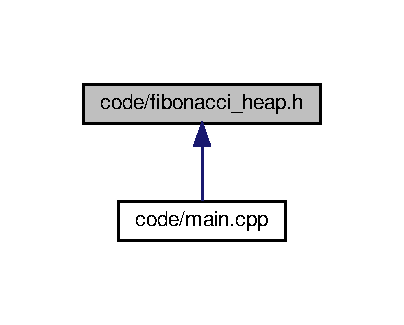
\includegraphics[width=194pt]{fibonacci__heap_8h__dep__incl}
\end{center}
\end{figure}
\subsection*{Classes}
\begin{DoxyCompactItemize}
\item 
struct \hyperlink{structnode}{node$<$ V $>$}
\item 
class \hyperlink{class_fibonacci_heap}{Fibonacci\+Heap$<$ V $>$}
\end{DoxyCompactItemize}

\hypertarget{main_8cpp}{}\section{dictionary/main.cpp File Reference}
\label{main_8cpp}\index{dictionary/main.\+cpp@{dictionary/main.\+cpp}}
{\ttfamily \#include \char`\"{}mainwindow.\+h\char`\"{}}\newline
{\ttfamily \#include $<$Q\+Application$>$}\newline
Include dependency graph for main.\+cpp\+:
\nopagebreak
\begin{figure}[H]
\begin{center}
\leavevmode
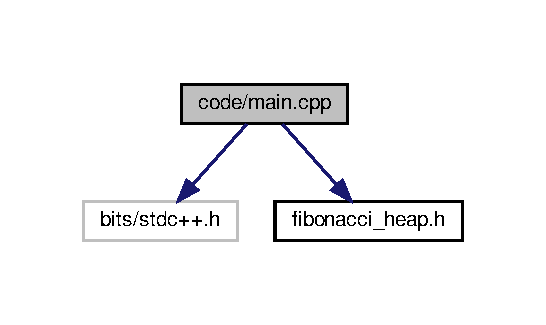
\includegraphics[width=250pt]{main_8cpp__incl}
\end{center}
\end{figure}
\subsection*{Functions}
\begin{DoxyCompactItemize}
\item 
int \hyperlink{main_8cpp_a0ddf1224851353fc92bfbff6f499fa97}{main} (int argc, char $\ast$argv\mbox{[}$\,$\mbox{]})
\end{DoxyCompactItemize}


\subsection{Function Documentation}
\mbox{\Hypertarget{main_8cpp_a0ddf1224851353fc92bfbff6f499fa97}\label{main_8cpp_a0ddf1224851353fc92bfbff6f499fa97}} 
\index{main.\+cpp@{main.\+cpp}!main@{main}}
\index{main@{main}!main.\+cpp@{main.\+cpp}}
\subsubsection{\texorpdfstring{main()}{main()}}
{\footnotesize\ttfamily int main (\begin{DoxyParamCaption}\item[{int}]{argc,  }\item[{char $\ast$}]{argv\mbox{[}$\,$\mbox{]} }\end{DoxyParamCaption})}



Definition at line 4 of file main.\+cpp.


%--- End generated contents ---

% Index
\backmatter
\newpage
\phantomsection
\clearemptydoublepage
\addcontentsline{toc}{chapter}{Index}
\printindex

\end{document}
